\documentclass[12pt,twoside]{article}

\newcommand{\reporttitle}{Reinforcement Learning}
\newcommand{\reportauthor}{Alexander Gaskell}
\newcommand{\reporttype}{Coursework 1}
\newcommand{\cid}{01813313}

% include files that load packages and define macros
%%%%%%%%%%%%%%%%%%%%%%%%%%%%%%%%%%%%%%%%%
% University Assignment Title Page 
% LaTeX Template
% Version 1.0 (27/12/12)
%
% This template has been downloaded from:
% http://www.LaTeXTemplates.com
%
% Original author:
% WikiBooks (http://en.wikibooks.org/wiki/LaTeX/Title_Creation)
%
% License:
% CC BY-NC-SA 3.0 (http://creativecommons.org/licenses/by-nc-sa/3.0/)
% 
% Instructions for using this template:
% This title page is capable of being compiled as is. This is not useful for 
% including it in another document. To do this, you have two options: 
%
% 1) Copy/paste everything between \begin{document} and \end{document} 
% starting at \begin{titlepage} and paste this into another LaTeX file where you 
% want your title page.
% OR
% 2) Remove everything outside the \begin{titlepage} and \end{titlepage} and 
% move this file to the same directory as the LaTeX file you wish to add it to. 
% Then add \input{./title_page_1.tex} to your LaTeX file where you want your
% title page.
%
%----------------------------------------------------------------------------------------
%	PACKAGES AND OTHER DOCUMENT CONFIGURATIONS
%----------------------------------------------------------------------------------------
\usepackage{ifxetex}
\usepackage{textpos}
\usepackage{natbib}
\usepackage{kpfonts}
\usepackage[a4paper,hmargin=2.8cm,vmargin=2.0cm,includeheadfoot]{geometry}
\usepackage{ifxetex}
\usepackage{stackengine}
\usepackage{tabularx,longtable,multirow,subfigure,caption}%hangcaption
\usepackage{fncylab} %formatting of labels
\usepackage{fancyhdr}
\usepackage{color}
\usepackage[tight,ugly]{units}
\usepackage{url}
\usepackage{float}
\usepackage[english]{babel}
\usepackage{amsmath}
\usepackage{graphicx}
\usepackage[colorinlistoftodos]{todonotes}
\usepackage{dsfont}
\usepackage{epstopdf} % automatically replace .eps with .pdf in graphics
\usepackage{natbib}
\usepackage{backref}
\usepackage{array}
\usepackage{latexsym}
\usepackage{etoolbox}

\usepackage{enumerate} % for numbering with [a)] format 



\ifxetex
\usepackage{fontspec}
\setmainfont[Scale=.8]{OpenDyslexic-Regular}
\else
\usepackage[pdftex,pagebackref,hypertexnames=false,colorlinks]{hyperref} % provide links in pdf
\hypersetup{pdftitle={},
  pdfsubject={}, 
  pdfauthor={\reportauthor},
  pdfkeywords={}, 
  pdfstartview=FitH,
  pdfpagemode={UseOutlines},% None, FullScreen, UseOutlines
  bookmarksnumbered=true, bookmarksopen=true, colorlinks,
    citecolor=black,%
    filecolor=black,%
    linkcolor=black,%
    urlcolor=black}
\usepackage[all]{hypcap}
\fi

\usepackage{tcolorbox}

% various theorems
\usepackage{ntheorem}
\theoremstyle{break}
\newtheorem{lemma}{Lemma}
\newtheorem{theorem}{Theorem}
\newtheorem{remark}{Remark}
\newtheorem{definition}{Definition}
\newtheorem{proof}{Proof}

% example-environment
\newenvironment{example}[1][]
{ 
\vspace{4mm}
\noindent\makebox[\linewidth]{\rule{\hsize}{1.5pt}}
\textbf{Example #1}\\
}
{ 
\noindent\newline\makebox[\linewidth]{\rule{\hsize}{1.0pt}}
}



%\renewcommand{\rmdefault}{pplx} % Palatino
% \renewcommand{\rmdefault}{put} % Utopia

\ifxetex
\else
\renewcommand*{\rmdefault}{bch} % Charter
\renewcommand*{\ttdefault}{cmtt} % Computer Modern Typewriter
%\renewcommand*{\rmdefault}{phv} % Helvetica
%\renewcommand*{\rmdefault}{iwona} % Avant Garde
\fi

\setlength{\parindent}{0em}  % indentation of paragraph

\setlength{\headheight}{14.5pt}
\pagestyle{fancy}
\fancyfoot[ER,OL]{\thepage}%Page no. in the left on
                                %odd pages and on right on even pages
\fancyfoot[OC,EC]{\sffamily }
\renewcommand{\headrulewidth}{0.1pt}
\renewcommand{\footrulewidth}{0.1pt}
\captionsetup{margin=10pt,font=small,labelfont=bf}


%--- chapter heading

\def\@makechapterhead#1{%
  \vspace*{10\p@}%
  {\parindent \z@ \raggedright %\sffamily
        %{\Large \MakeUppercase{\@chapapp} \space \thechapter}
        %\\
        %\hrulefill
        %\par\nobreak
        %\vskip 10\p@
    \interlinepenalty\@M
    \Huge \bfseries 
    \thechapter \space\space #1\par\nobreak
    \vskip 30\p@
  }}

%---chapter heading for \chapter*  
\def\@makeschapterhead#1{%
  \vspace*{10\p@}%
  {\parindent \z@ \raggedright
    \sffamily
    \interlinepenalty\@M
    \Huge \bfseries  
    #1\par\nobreak
    \vskip 30\p@
  }}
  



% %%%%%%%%%%%%% boxit
\def\Beginboxit
   {\par
    \vbox\bgroup
	   \hrule
	   \hbox\bgroup
		  \vrule \kern1.2pt %
		  \vbox\bgroup\kern1.2pt
   }

\def\Endboxit{%
			      \kern1.2pt
		       \egroup
		  \kern1.2pt\vrule
		\egroup
	   \hrule
	 \egroup
   }	

\newenvironment{boxit}{\Beginboxit}{\Endboxit}
\newenvironment{boxit*}{\Beginboxit\hbox to\hsize{}}{\Endboxit}



\allowdisplaybreaks

\makeatletter
\newcounter{elimination@steps}
\newcolumntype{R}[1]{>{\raggedleft\arraybackslash$}p{#1}<{$}}
\def\elimination@num@rights{}
\def\elimination@num@variables{}
\def\elimination@col@width{}
\newenvironment{elimination}[4][0]
{
    \setcounter{elimination@steps}{0}
    \def\elimination@num@rights{#1}
    \def\elimination@num@variables{#2}
    \def\elimination@col@width{#3}
    \renewcommand{\arraystretch}{#4}
    \start@align\@ne\st@rredtrue\m@ne
}
{
    \endalign
    \ignorespacesafterend
}
\newcommand{\eliminationstep}[2]
{
    \ifnum\value{elimination@steps}>0\leadsto\quad\fi
    \left[
        \ifnum\elimination@num@rights>0
            \begin{array}
            {@{}*{\elimination@num@variables}{R{\elimination@col@width}}
            |@{}*{\elimination@num@rights}{R{\elimination@col@width}}}
        \else
            \begin{array}
            {@{}*{\elimination@num@variables}{R{\elimination@col@width}}}
        \fi
            #1
        \end{array}
    \right]
    & 
    \begin{array}{l}
        #2
    \end{array}
    &%                                    moved second & here
    \addtocounter{elimination@steps}{1}
}
\makeatother

%% Fast macro for column vectors
\makeatletter  
\def\colvec#1{\expandafter\colvec@i#1,,,,,,,,,\@nil}
\def\colvec@i#1,#2,#3,#4,#5,#6,#7,#8,#9\@nil{% 
  \ifx$#2$ \begin{bmatrix}#1\end{bmatrix} \else
    \ifx$#3$ \begin{bmatrix}#1\\#2\end{bmatrix} \else
      \ifx$#4$ \begin{bmatrix}#1\\#2\\#3\end{bmatrix}\else
        \ifx$#5$ \begin{bmatrix}#1\\#2\\#3\\#4\end{bmatrix}\else
          \ifx$#6$ \begin{bmatrix}#1\\#2\\#3\\#4\\#5\end{bmatrix}\else
            \ifx$#7$ \begin{bmatrix}#1\\#2\\#3\\#4\\#5\\#6\end{bmatrix}\else
              \ifx$#8$ \begin{bmatrix}#1\\#2\\#3\\#4\\#5\\#6\\#7\end{bmatrix}\else
                 \PackageError{Column Vector}{The vector you tried to write is too big, use bmatrix instead}{Try using the bmatrix environment}
              \fi
            \fi
          \fi
        \fi
      \fi
    \fi
  \fi 
}  
\makeatother

\robustify{\colvec}

%%% Local Variables: 
%%% mode: latex
%%% TeX-master: "notes"
%%% End: 
 % various packages needed for maths etc.
% quick way of adding a figure
\newcommand{\fig}[3]{
 \begin{center}
 \scalebox{#3}{\includegraphics[#2]{#1}}
 \end{center}
}

%\newcommand*{\point}[1]{\vec{\mkern0mu#1}}
\newcommand{\ci}[0]{\perp\!\!\!\!\!\perp} % conditional independence
\newcommand{\point}[1]{{#1}} % points 
\renewcommand{\vec}[1]{{\boldsymbol{{#1}}}} % vector
\newcommand{\mat}[1]{{\boldsymbol{{#1}}}} % matrix
\newcommand{\R}[0]{\mathds{R}} % real numbers
\newcommand{\Z}[0]{\mathds{Z}} % integers
\newcommand{\N}[0]{\mathds{N}} % natural numbers
\newcommand{\nat}[0]{\mathds{N}} % natural numbers
\newcommand{\Q}[0]{\mathds{Q}} % rational numbers
\ifxetex
\newcommand{\C}[0]{\mathds{C}} % complex numbers
\else
\newcommand{\C}[0]{\mathds{C}} % complex numbers
\fi
\newcommand{\tr}[0]{\text{tr}} % trace
\renewcommand{\d}[0]{\mathrm{d}} % total derivative
\newcommand{\inv}{^{-1}} % inverse
\newcommand{\id}{\mathrm{id}} % identity mapping
\renewcommand{\dim}{\mathrm{dim}} % dimension
\newcommand{\rank}[0]{\mathrm{rk}} % rank
\newcommand{\determ}[1]{\mathrm{det}(#1)} % determinant
\newcommand{\scp}[2]{\langle #1 , #2 \rangle}
\newcommand{\kernel}[0]{\mathrm{ker}} % kernel/nullspace
\newcommand{\img}[0]{\mathrm{Im}} % image
\newcommand{\idx}[1]{{(#1)}}
\DeclareMathOperator*{\diag}{diag}
\newcommand{\E}{\mathds{E}} % expectation
\newcommand{\var}{\mathds{V}} % variance
\newcommand{\gauss}[2]{\mathcal{N}\big(#1,\,#2\big)} % gaussian distribution N(.,.)
\newcommand{\gaussx}[3]{\mathcal{N}\big(#1\,|\,#2,\,#3\big)} % gaussian distribution N(.|.,.)
\newcommand{\gaussBig}[2]{\mathcal{N}\left(#1,\,#2\right)} % see above, but with brackets that adjust to the height of the arguments
\newcommand{\gaussxBig}[3]{\mathcal{N}\left(#1\,|\,#2,\,#3\right)} % see above, but with brackets that adjust to the height of the arguments
\DeclareMathOperator{\cov}{Cov} % covariance (matrix) 
\ifxetex
\renewcommand{\T}[0]{^\top} % transpose
\else
\newcommand{\T}[0]{^\top}
\fi
% matrix determinant
\newcommand{\matdet}[1]{
\left|
\begin{matrix}
#1
\end{matrix}
\right|
}



%%% various color definitions
\definecolor{darkgreen}{rgb}{0,0.6,0}

\newcommand{\blue}[1]{{\color{blue}#1}}
\newcommand{\red}[1]{{\color{red}#1}}
\newcommand{\green}[1]{{\color{darkgreen}#1}}
\newcommand{\orange}[1]{{\color{orange}#1}}
\newcommand{\magenta}[1]{{\color{magenta}#1}}
\newcommand{\cyan}[1]{{\color{cyan}#1}}


% redefine emph
\renewcommand{\emph}[1]{\blue{\bf{#1}}}

% place a colored box around a character
\gdef\colchar#1#2{%
  \tikz[baseline]{%
  \node[anchor=base,inner sep=2pt,outer sep=0pt,fill = #2!20] {#1};
    }%
}%
 % short-hand notation and macros

\usepackage[export]{adjustbox}
\usepackage[T1]{fontenc}
\usepackage[scaled]{beramono}
\usepackage{listings}

%%%%%%%%%%%%%%%%%%%%%%%%%%%%

\begin{document}
% front page
% % Last modification: 2016-09-29 (Marc Deisenroth)
\begin{titlepage}

\newcommand{\HRule}{\rule{\linewidth}{0.5mm}} % Defines a new command for the horizontal lines, change thickness here


%----------------------------------------------------------------------------------------
%	LOGO SECTION
%----------------------------------------------------------------------------------------


\includegraphics[width = 4cm]{./figures/imperial}\\[0.5cm] 

\begin{center} % Center remainder of the page

%----------------------------------------------------------------------------------------
%	HEADING SECTIONS
%----------------------------------------------------------------------------------------
\textsc{\LARGE \reporttype}\\[1.5cm] 
\textsc{\Large Imperial College London}\\[0.5cm] 
\textsc{\large Department of Computing}\\[0.5cm] 
%----------------------------------------------------------------------------------------
%	TITLE SECTION
%----------------------------------------------------------------------------------------

\HRule \\[0.4cm]
{ \huge \bfseries \reporttitle}\\ % Title of your document
\HRule \\[1.5cm]
\end{center}
%----------------------------------------------------------------------------------------
%	AUTHOR SECTION
%----------------------------------------------------------------------------------------

%\begin{minipage}{0.4\hsize}
\begin{flushleft} \large
\textit{Author:}\\
\reportauthor~(CID: \cid) \\% Your name 
\textit{Email:} \\
\reportemail
\end{flushleft}
\vspace{2cm}
\makeatletter
Date: \@date 

\vfill % Fill the rest of the page with whitespace



\makeatother


\end{titlepage}




%%%%%%%%%%%%%%%%%%%%%%%%%%%% Main document
\textbf{Alexander Gaskell, CID = 01813313, aeg19@imperial.ac.uk} \\

\textbf{Understanding of MDPs (20 points)} \\

\textbf{1.1}
\begin{align}
    \tau = s_01s_10s_01s_21s_21s_01s_21 \quad [CID = 01813313] \label{trace}
\end{align}

\textbf{1.2 a)}

\begin{figure}[h]
\centering % this centers  the figure
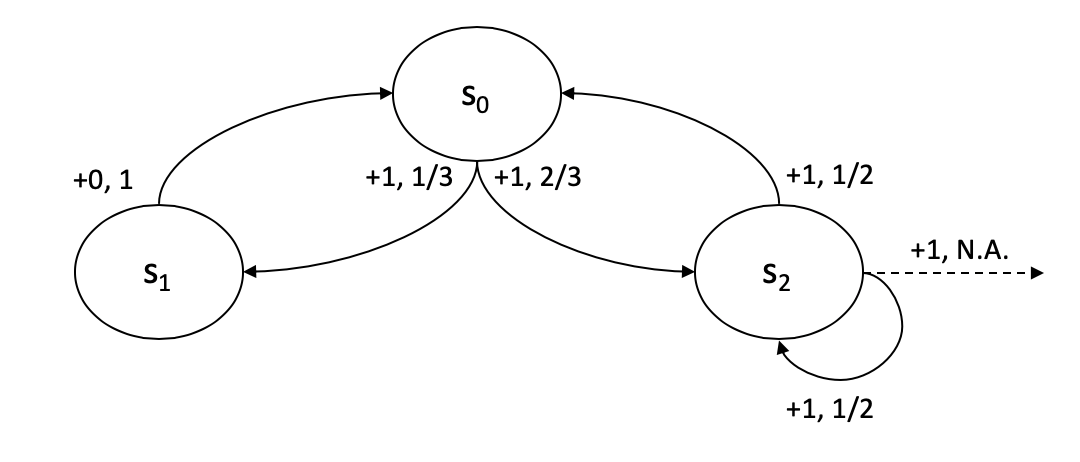
\includegraphics[width = 0.6\hsize]{./figures/min_MDP.png}
\caption{The minimal MDP graph as given by the trace in equation \ref{trace}.} % caption of the figure
\label{MDP}
\end{figure}

The minimal MDP above represents the trace given in equation \ref{trace}. The graph contains 3 states $\{s_0,s_1,s_2\}$ and the arrows represent transitions from state $s$ to $s'$. Next to each arrow are two numbers: the first represents the reward (I assume the reward is for the transition from state $s$ to $s'$ ($\mathcal{R}^a_{ss'}$)); the second represents the probability of transitioning to state s' given the agent is in state s ($\mathcal{P}^a_{ss'}$). The absence of arrows connecting $s_1$ and $s_2$ reflects there being no transition observed between the two states. As I have assumed rewards are related to transitions (rather than states), the final reward in the trace implies this trace is incomplete. Therefore, the final reward is represented by the dotted line in the graph.\\

In this graph I assume that the transition probabilities and rewards are representative of the environment; clearly these assumptions may not withstand observing more data. The transition matrix is stochastic given the data because the agent transitions to both $s_1$ and $s_2$ from $s_0$, and to both $s_2$ and $s_0$ from $s_2$. Additionally, the reward function is deterministic: the only transition the agent repeats is $s_0$ to $s_2$, and this gives $+1$ reward both times. Clearly this assumption may not withstand observing more data as it is based upon a single data point. \\

\textbf{1.2 b)} The choice of method for computing the value of $s_0$ hinges upon the set of assumptions. A straightforward method of computing $V(s_0)$ would be to assume that we are in an MRP and invert the Bellman equation to solve for all state values. However, this would require a prohibitively strong set of assumptions to be valid (such as the trace perfectly representing the environment and the presence of some terminal state). Additionally, I have assumed the trace is incomplete (see 1.a), so Monte Carlo would also be inappropriate.\\ 

We can use temporal difference learning to compute $V(s_0)$ as this does not require any assumptions (aside the learning rate). TD learns directly after each episode and uses bootstrapping to learn at each step. Additionally, TD does not require knowledge of the reward function or state transition probabilities, so we do not need to assume the world is perfectly summarized by figure \ref{MDP}. This works as follows:
\begin{align}
    V(s_t) \leftarrow V(s_t) + \alpha(r_{t+1} + \gamma V(S_{t+1}) - V(S_t))
    \label{eq:TD}
\end{align}
$V(s_t)$ is the value of the current state, $V(s_{t+1})$ is the value of the following state, $r_{t+1}$ is the reward observed, $\alpha$ is the learning rate and $\gamma$ is the discount rate. We begin by initialising all $V(s)$ to zero. We then update the state values by iterating through the trace and computing equation \ref{eq:TD} at each step. $\alpha$ is the learning rate which determines how much the agent learns from new experiences. (To simplify the algebra,) I will set $\alpha = 0.5$, with 0.5 satisfying the Robinson-Monroe sequence.
\begin{align}
    & t = 1: \quad V(s_0) \leftarrow 0 + \frac{1}{2}(1+\gamma *0-0) = \frac{1}{2} \quad \quad [s_t = s_0, s_{t+1}=s_1]\\
    & t = 2: \quad V(s_1) \leftarrow 0 + \frac{1}{2}(0+ \gamma*\frac{1}{2}  - 0) = \frac{\gamma}{4} \quad \quad [s_t = s_1, s_{t+1}=s_0]\\
    & t = 3: \quad V(s_0) \leftarrow \frac{1}{2} + \frac{1}{2}(1+\gamma*0 - \frac{1}{2}) = \frac{3}{4} \quad \quad [s_t = s_0, s_{t+1}=s_2]\\
    & t = 4: \quad V(s_2) \leftarrow 0 + \frac{1}{2}(1+\gamma*0 -0) = \frac{1}{2} \quad \quad [s_t = s_2, s_{t+1}=s_2]\\
    & t = 5: \quad V(s_2) \leftarrow \frac{1}{2} + \frac{1}{2} (1+\gamma*\frac{3}{4} - \frac{1}{2}) = \frac{3}{8}(\gamma +2) \quad \quad [s_t = s_2, s_{t+1}=s_0]\\
    & t = 6: V(s_0) \leftarrow \frac{3}{4} + \frac{1}{2} (1+\gamma*\frac{3}{8}(\gamma +2)-\frac{3}{4}) = \frac{14 + 3\gamma (\gamma + 2)}{16}  \quad [s_t = s_0, s_{t+1}=s_2] \label{eq:s_0}
\end{align}
Using $\gamma=1$, from equation \ref{eq:s_0} we compute the $V(s_0)=1.44$ (3 s.f.).\\






\textbf{2. Understanding of Grid Worlds (20 points)} \\

\textbf{2.1} Given the final 3 digits of my CID are 313, $x=3, y=1, z=3$.
\begin{align}
    s_j = s_2 \quad p =0.4 \quad \gamma = 0.25
\end{align}

\textbf{2.2} I computed the optimal value function and optimal policy by using policy iteration (code attached for reference); these are illustrated in figures \ref{Optimal policy} and \ref{Optimal value function}. I solved the problem using dynamic programming (policy iteration) as follows:
\begin{enumerate}
    \item Initialized the policy by setting the probability of any action in any state $= 0.25$ and initialise the value function at some value
    \item Perform policy evaluation to compute the state value function given this policy. This uses the Bellman Expectation Equation to compute the state value function:
    \begin{align}
        V(s) = \sum_a \pi(s,a) \sum_{s'} \mathcal{P}^a_{ss'} (\mathcal{R}^a_{ss'} + \gamma V(s'))
    \end{align}
    This says, given the agent is in a state s, the value of state s is a function of the policy $\pi(s,a)$, the probability of moving to another state given an action ($\mathcal{P}^a_{ss'}$), the expected value of all other states, a discounting factor $\gamma$ and an immediate reward (or penalty) based on the transition $\mathcal{R}^a_{ss'}$. This reward is 10 if the agent is transitioning to $s_2$, -100 if transitioning to $s_{11}$, and 0 otherwise. Policy evaluation iteratively computes the value of all states until the values converge. Convergence is defined as being when the difference between updated and original values is below some threshold (a hyper-parameter; $10^{-6}$ in this case).
    \item Given the value function computed above, perform policy improvement to find the optimal policy for each state. This means, for each state, set the policy to 1 to perform the action that gives the highest value and 0 for all other actions.
    \item Iteratively perform the above 2 steps until the state value function and policy converge to their optimum. Similar to the above, convergence is defined by the value function moving less than the threshold hyper-parameter.
\end{enumerate}

\begin{figure}[h]
    \centering
    \begin{minipage}[t]{0.35\textwidth}
        \centering % this centers the figure
        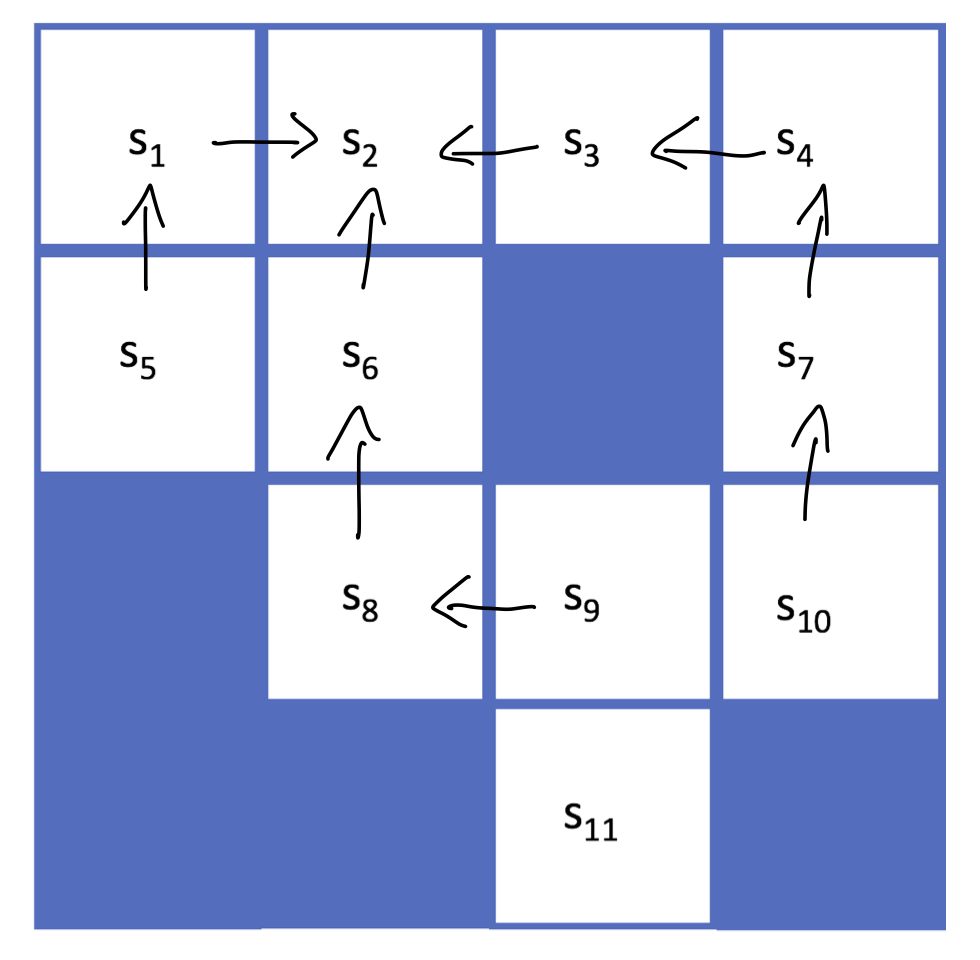
\includegraphics[width = 0.9\hsize]{./figures/Optimal_policy.png}
        \caption{The optimal policy. \textbf{Note}: I have not drawn optimal policies for $s_2$ and $s_{11}$ (terminal states).}
        \label{Optimal policy}
    \end{minipage}\hfill
    \begin{minipage}[t]{0.35\textwidth}
        \centering % this centers the figure
        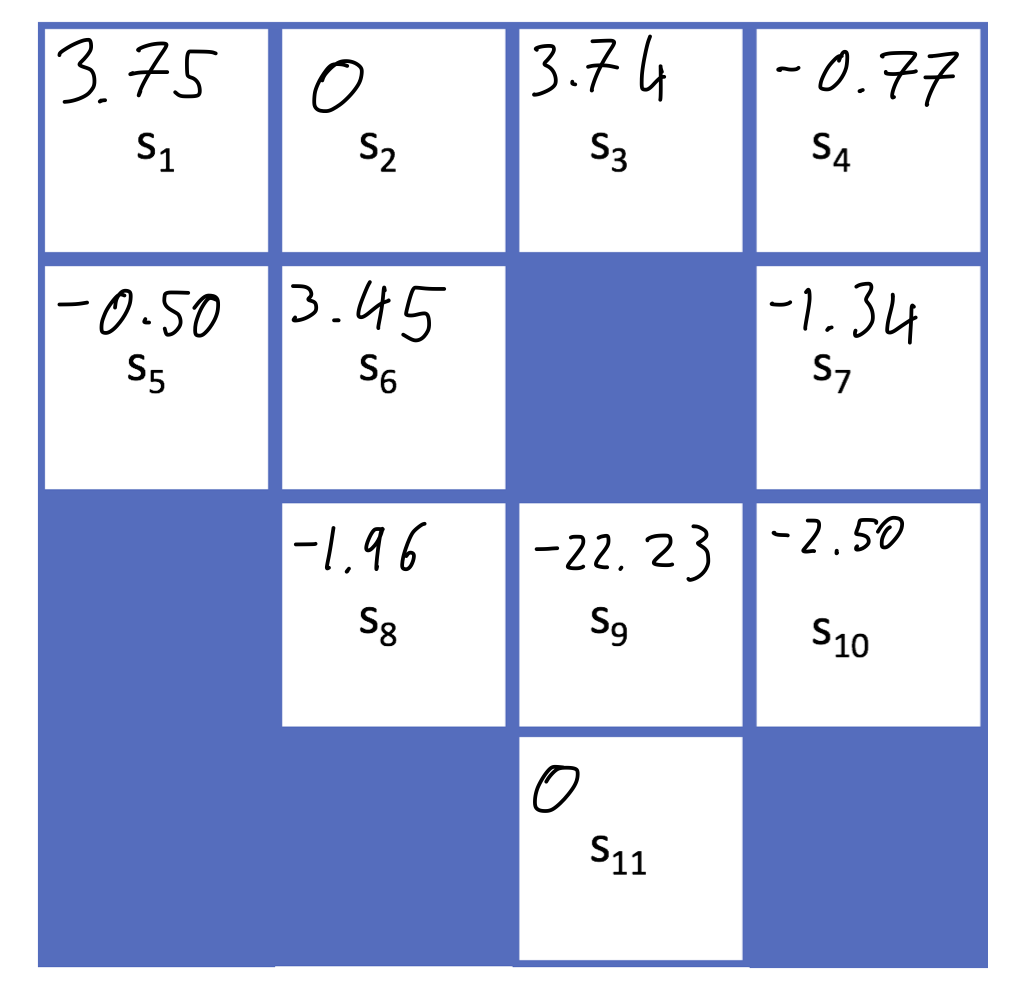
\includegraphics[width = 0.9\hsize]{./figures/Optimal_state_values.png}
        \caption{The optimal value function}
        \label{Optimal value function}
    \end{minipage}
\end{figure}


\textbf{2.3} The optimal policy dictates the agent should move west if it is in $s_9$ (explicitly speaking, move west with probability of 1 and move in every other direction with probability of 0). This means $p(a,s_9) = (0.2, 0.2, 0.2, 0.4)$ (where actions are (N,E,S,W)). This makes intuitive sense as the game only end when the agent reaches $s_2$ or $s_{11}$ and $s_2$ is the reward state, so the agent should move toward $s_2$. \\

The agent chooses to move west instead of east at $s_9$. This also makes sense for two reasons: there is a transition cost of -1 for each movement and the discount factor is less than one, meaning for each period the agent is delayed, the reward of reaching $s_2$ falls. These two factors mean the agent will take the shortest path to $s_2$, hence the optimal policy for the agent at $s_9$ is to move west. \\

The choice of $\gamma$ does have an impact on the optimal policy at $s_9$. In the special case of $\gamma=0$, the agent is myopic and does not consider any rewards aside from immediate rewards. In this instance, the agent is indifferent between moving north, east and west as all have a cost of one; the agent simply wants to avoid the penalty of reaching $s_{11}$. If $\gamma$ is close to 1, however, the optimal policy is unchanged as the agent still wants to take the shortest path to $s_2$ to avoid the transition costs.\\

The choice of $p$ also has an impact: while $p>0.25$, the optimal policy remains to move west. However, if $p=0.25$, then any policy would be the optimal policy as the transition would be completely stochastic so the choice of policy would have not impact on which state the agent ends up in. If $p<0.25$, the optimal policy would be to move south; in this case, the probability of actually moving south (given the agent chose the action south) is lower than the probability of moving in any other direction, so the optimal policy would be to choose south.\\

\textbf{2.4} As explained above, the optimal policy always points towards $s_2$ and away from $s_{11}$ as the agent wants to receive the reward for $s_2$ in as few transitions as possible, and to avoid the penalty of $s_{11}$, as illustrated in figure \ref{Optimal policy}. This can be seen in the optimal value function in figure \ref{Optimal value function}, with states closest to $s_2$ having the highest values and cells closest to $s_{11}$ having the lowest values. If we assume the both $\gamma$ and $p$ are between 0 and 1, then this observation is independent of the choice of $\gamma$ and $p$. In question 2.3 I have addressed the special cases of where $\gamma = 0$ and $p \leq 0.25$.\\

Another noticeable feature of the optimal state values are that they are much smaller than the reward/penalties the terminal states, and are more likely to be negative than positive (both the median and mean state values of non-terminating states are negative). This is largely due to the negative penalty for arriving at $s_{11}$ and the transition cost, but $\gamma$ and $p$ do have an effect. If this grid-world was deterministic (i.e. the probability of moving a certain direction given the action of moving that direction was 1), then the optimal state values would be strictly positive (assuming $\gamma$ is high enough, specifically $\gamma \geq 0.6$) as the risk of falling into $s_{11}$ would be zero under the optimal policy, and also the agent can ensure it takes the most direct route to $s_2$ (no movements in directions which are not the desired direction), hence the only penalty is the transition cost. \\

Additionally, if $\gamma$ is higher (close to 1), the optimal state values would increase in magnitude (meaning states close to $s_{11}$ would become more negative. This is because the discount works to lessen the reward from reaching the terminal state, so if no discount is applied then the impact of reaching the terminal states is increased. This change works to polarise the state values in grid-world further: states close to $s_2$ would see their values rise, but states close to $s_{11}$ would see their values fall.\\

To conclude, the choices of $\gamma$ and $p$ have a large impact on the size and distribution of the optimal state values. They have less of of an impact on the optimal policy as the agent still wants to avoid the transition cost, so the optimal policy remains to move toward $s_2$ using the shortest path irrespective of the values of $\gamma$ and $p$ (except for some special cases as addressed in question 2.3).



\newpage

\section{Appendix: code for GridWorld}

\begin{verbatim}
import numpy as np
import matplotlib.pyplot as plt

class GridWorld:

    def __init__(self, gamma=0.25, p=0.4, threshold=10**-6):
        self.gamma = gamma
        self.p = p
        self.states = 11
        self.threshold = threshold
        self.terminal_states = [1,10]

        self.dict_transitions, self.t_m = self.build_transition_matrix()
        self.reward_fun = self.get_rewards()

    def build_transition_matrix(self):
        '''
        :return dict_transitions: dictionary showing, 
        for each grid, where the agent would end up if 
        it moved in a direction
        :return transition_matrix: creates transition 
        matrix (11x11x4 tensor) showing probability 
        of moving to a different state from the agent's 
        current state given an action. The action is 
        stochastic with probability p of success.
        '''
        # Format: current_grid:[N,E,S,W]
        dict_transitions = {
            1:np.array([1,2,5,1]),
            2:np.array([2,2,2,2]),        # Terminal state
            3:np.array([3,4,3,2]),
            4:np.array([4,4,7,3]),
            5:np.array([1,6,5,5]),
            6:np.array([2,6,8,5]),
            7:np.array([4,7,10,7]),
            8:np.array([6,9,8,8]),
            9:np.array([9,10,11,8]),
            10:np.array([7,10,10,9]),
            11:np.array([11,11,11,11])       # Terminal state
        }

        transition_matrix = np.zeros((self.states,self.states,4))

        for k,vals in dict_transitions.items():
            for n,v in enumerate(vals):
                transition_matrix[k-1,v-1,n] += self.p        

                for i in range(1,4):
                    transition_matrix[k-1,v-1,(n+i)%4] += (1-self.p)/3        

        assert (np.sum(transition_matrix, axis = 1) - 1 < 0.01).all(),\
        "Probabilites do not sum to 1"

        return dict_transitions, transition_matrix

    def get_rewards(self):
        '''
        Assumes 0 reward for every state except the terminal states
        '''
        rewards = {1:-1,2:10,3:-1,4:-1,5:-1,6:-1,7:-1,8:-1,9:-1,\
        10:-1,11:-100}
        return list(rewards.values())

    def compute_value_fn(self, policy, value_fn):
        '''
        Uses the Bellman equation to compute the value function for each 
        state given a policy.
        Assumes that the transition cost is not discounted (& is
        replaced by the rewards of the transition states
        if transitioning to the terminal_states)

        :return updated_value_fn: array containing new value function
        '''
        updated_value_fn = np.zeros((self.states,))

        for s in range(self.states):
            if s in self.terminal_states:
                updated_value_fn[s] = value_fn[s]
            else:
                transition_ps = np.sum([p*self.t_m[s,:,n] for n,p \
                in enumerate(policy[s])], axis=0)
                # Bellman equation
                val = sum([t_p*(R + self.gamma*val) if R not in \
                [-100, 10] else t_p*R for t_p,val,R in \
                zip(transition_ps, value_fn, self.reward_fun)])      
                updated_value_fn[s] = val

        return updated_value_fn

    def policy_evaluation(self, policy, value_fn):
        '''
        Iteratively evaluates a given policy until the value
        function stabilises

        :return value_fn: updated value function evaluated at the policy
        '''
        delta = 2*self.threshold        # Init delta at above the threshold

        while delta > self.threshold:

            value_fn_old = value_fn.copy()
            value_fn = self.compute_value_fn(policy, value_fn)

            delta = max(abs(value_fn-value_fn_old))

        return value_fn

    def improve_policy(self, policy, value_fn):
        '''
        Given a value function, compute the optimal policy (i.e. 
        for each state, find the adjacent state with the 
        highest value, and set the policy to moving to this cell).

        :return P: an optimal policy (11x4 array) given the value function
        '''
        P = policy.copy()
        for i,p in enumerate(list(self.dict_transitions.values())):
            if i not in self.terminal_states:
                argmax_p = np.argmax([value_fn[int(j)-1] for j in p])
                P[i] = np.zeros((4,))
                P[i,argmax_p] = 1
        return P

    def policy_iteration(self):
        '''
        Perform policy iteration to find an optimal policy and 
        optimal state value function.

        Method:
        - Init the policy randomly and the value function to 
        the state rewards
        - Perform policy evaluation to get value function 
        given policy
        - Perform policy improvement to get optimal policy 
        given value function
        - Repeat the above 2 steps until the state function 
        stabilises

        :return policy: optimal policy (11x4)
        :return value_fn: optimal state value function (11,)
        :return epochs: # iterations until convergence
        '''
        # Begin with a random policy
        policy = np.ones((11,4))/4 
        # Init value function to the rewards
        value_fn = np.array(self.reward_fun)        

        delta = 2*self.threshold        # Init delta at above the threshold

        epochs = 0
        while delta > self.threshold:
            value_fn_old = value_fn.copy()      
            value_fn = self.policy_evaluation(policy, value_fn)
            policy = self.improve_policy(policy, value_fn)

            epochs += 1     # Track convergence epochs

            delta = max(abs(value_fn-value_fn_old))

        for i in self.terminal_states:         
            value_fn[i] = 0

        return policy, value_fn, epochs

    def main(self):
        '''
        For running GridWorld methods
        '''
        optimal_policy, optimal_value_fn, epochs = self.policy_iteration()
        print(optimal_policy)
        print(optimal_value_fn)
        print(epochs)


if __name__ == '__main__':
    np.set_printoptions(precision = 3)
    grid = GridWorld()
    grid.main()
\end{verbatim}













\end{document}
%%% Local Variables: 
%%% mode: latex
%%% TeX-master: t
%%% End: 
